\chapter*{Bilagor}
\addcontentsline{toc}{chapter}{Bilagor}
\appendix

\chapter{Att koppla upp sig mot SALSA med programmet Nomachine 4}
\label{app:nomachine}
Programmet NoMachine kan användas för att koppla upp sig till datorerna som
kontrollerar SALSA-teleskopen. Denna guide gjordes med version 4 av NoMachine,
, hämtat från http://www.nomachine.com. NoMachine-programmet fungerar på Windows,
Mac eller Linux så du bör kunna styra SALSA från nästan vilken dator som helst. 
Om du, när du försöker använda denna guide, märker att instruktionerna inte passar
med vad du ser på skärmen så beror det troligen på att NoMachine-programmet har 
ändrats utan att vi uppdaterat guiden. Isåfall, vänligen meddela SALSA-support 
(se SALSA-hemsidan) så att vi kan uppdatera denna guide.

\section{Guide: steg för steg}
I detta exempel så ansluter vi till en SALSA-dator som kallas \emph{vale}.
\begin{enumerate}
	\item Ladda först hem och installera programmet NoMachine som finns gratis
		på hemsidan http://www.nomachine.com. 
\item När NoMachine är installerat, öppna en webbläsare och gå till SALSA-hemsidan 
	http://vale.oso.chalmers.se. På sidan "Software" så finns ett stycke om 
	NoMachibe. I detta stycke finns en länk till en fil som heter "SALSA-Vale.nxs.
	Spara ner denna fil till din dator (använd höger-klick och välj Spara länk som).
	Obs: Om du har en Mac, försäkra dig om att filen sparas korrekt utan att något
	extra till filens namn.
\item Öppna filen SALSA-Vale.nxs, antingen genom att dubbelklicka på filen, eller genom
	att starta NoMachine-programmet och använd knappen "Open" för att öppna filen. 
	Du kanske nu ser lite välkomstinformation från NoMachine, klicka bara OK tills du
	kan skriva in användarnamn och lösenord, alltså du ser något liknande Fig. 
	\ref{fig:login}. (Om du får en fråga om att "Verify host authenticity", svara 
	\emph{Yes}.)
\begin{figure}[H]
    \centering
    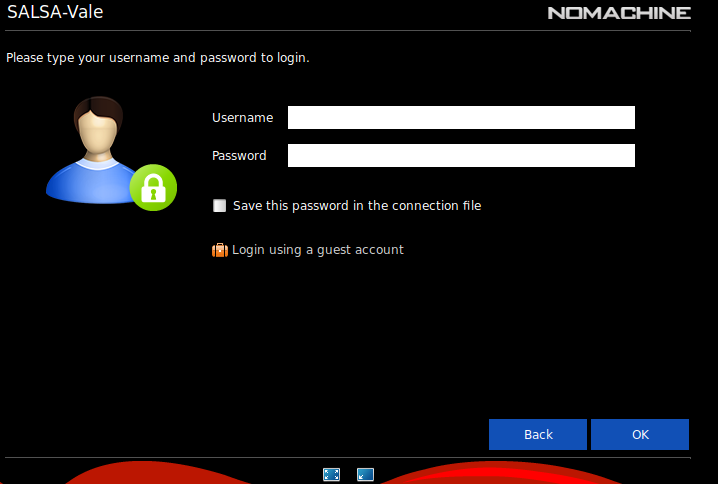
\includegraphics[height=0.5\textwidth]{../figures/nomachinefigs/SALSA_login.png}
    \caption{Vänligen skriv in ditt SALSA-användarnamn och telescope password.}
    \label{fig:login}
\end{figure}
\item Vänligen skriv in ditt SALSA användarnamn och telescope password och klicka OK. 
	Du kanske igen får se lite information från Nomachine, du kan bara klicka OK
	på dessa bilder. 
{\bf Obs:} Här måste du använda ditt ``telescope password'', som kan vara annorlunda än 
det lösenord som du använder för att boka observationstid. Kolla på SALSA-hemsidan, under
``My account'' för att hitta ditt telescope password. Kom även ihåg att du bara kan ansluta
till SALSA-datorn om du har bokat observationstid. 
\item Några användare frågas om olika val för att "Create a new virtual desktop", se 
	Fig. \ref{fig:virtual}. Om du får dessa val, välj GNOME-alternativet och klicka continue.
\begin{figure}[H]
    \centering
    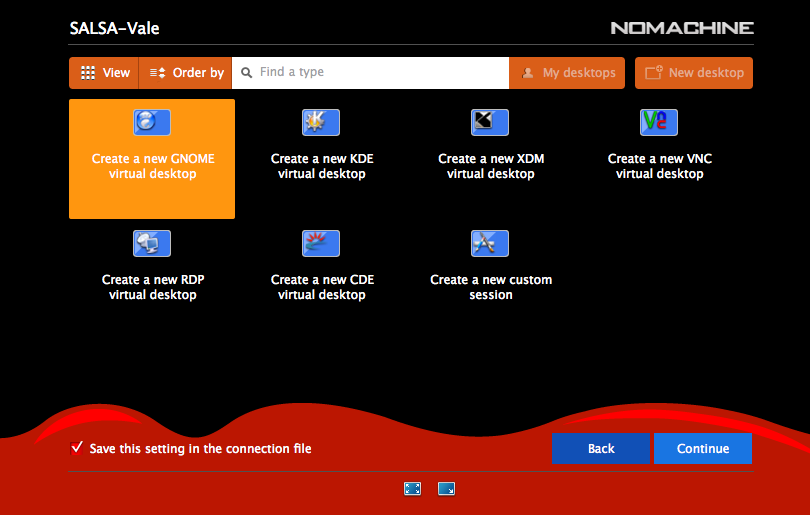
\includegraphics[height=0.5\textwidth]{../figures/nomachinefigs/fig_virtual.png}
	\caption{Om du ser denna eller en liknande skärmbild (det gäller inte alla användare)
		välj GNOME och klicka på continue.
	}
    \label{fig:virtual}
\end{figure}
\item Du bör nu vara uppkopplad till datorn Vale och du bör se ett fönster på skärmen 
	med ett virtuellt skrivbord, som om du satt framför datorn Vale, se Fig. 
	\ref{fig:connected}.  Du kanske vill maximera fönstret för att se hela skrivbordet.
\item Nu kan du starta SALSA-programmet genom att dubbelklicka på SALSA-ikonen på
	skrivbordet. {\bf Obs}: Om du inte kan se hela SALSA-programmet, 
	(som i Fig. \ref{fig:toosmall}) så kan du behöva ändra skärmupplösning,
	se avsnitt 	\ref{sect:screenres} nedan.
\end{enumerate}

\begin{figure}[H]
    \centering
	
\includegraphics[width=0.9\textwidth]{../figures/nomachinefigs/fig9-connected.pdf}
	\caption{Nu ser du förhoppningsvis, kanske efter några välkomstbilder från
		NoMachine, något liknande detta på skärmen. Grattis - du är nu
		uppkopplad mot SALSA och du kan börja observera! För att styra
		teleskopet, dubbelklicka på genvägen SALSA på skrivbordet. {\bf Obs}:
		Om du inte kan se hela SALSA-programmet, (som i Fig.
		\ref{fig:toosmall}) så kan du behöva ändra skärmupplösning, se avsnitt
		\ref{sect:screenres} nedan.
} 
\label{fig:connected} 
\end{figure}

\section{Felsökning: att öka kontrolldatorns skärmupplösning}
\label{sect:screenres}
Vissa användare som ansluter till SALSA med NoMachine kommer som standard
att få ett fönster som är så litet att de inte kan se den nedre delan av kontrollprogrammet.
Detta innebär att de inte kan se knapparna under spektrum-fönstret, som i Fig. \ref{fig:toosmall}, 
inklusive det område där de kan läsa av koordinaterna under muspekaren. 
Dessutom så kanske de inte kan se Upload-knappen och kan därmed inte spara sina mätningar. 
Detta kan åtgärdas genom att öka skärmupplösningen för kontrolldatorn. För att göra detta,
följ stegen i figurerna \ref{fig:controlcenter} och \ref{fig:monitors}.

\begin{figure}[H]
    \centering
    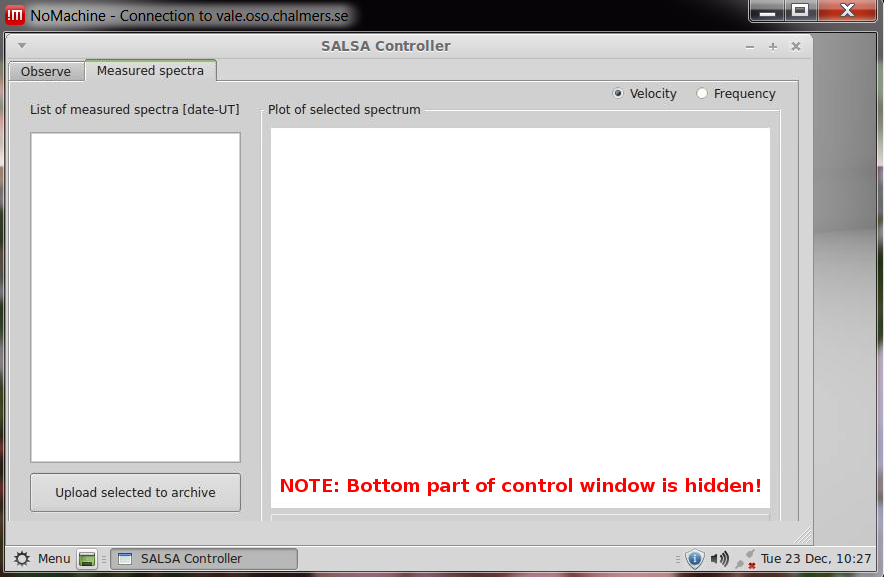
\includegraphics[height=0.3\paperheight]{../figures/nomachinefigs/fig9_toosmallwin.png}
    \caption{För vissa användare så är NoMachine-fönstret för litet, vilket innebär att vissa
		delar av kontrollprogrammet inte kan visas korrekt. För att åtgärda detta så kan du
		öka skärmupplösningen på kontrolldatorn.}
    \label{fig:toosmall}
\end{figure}

\begin{figure}[H]
    \centering
    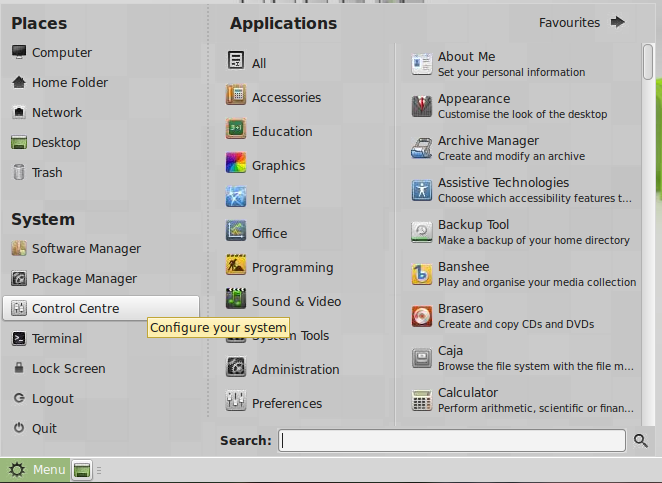
\includegraphics[height=0.3\paperheight]{../figures/nomachinefigs/fig10_menu.png}
	\caption{För att ändra skärmupplösning, klicka först på knappen \emph{Menu} nere till
		vänster på ditt virtuella skrivbord (d.v.s. inne i NoMachine-fönstret). 
		Klicka därefter på \emph{Control center}. Inne i Control center, klicka på \emph{Monitors}.}
    \label{fig:controlcenter}
\end{figure}

\begin{figure}[H]
    \centering
    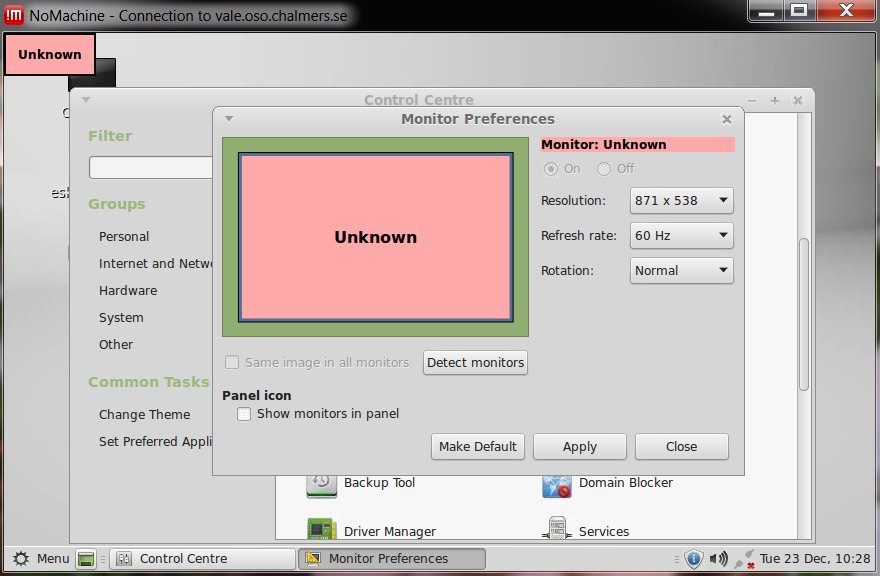
\includegraphics[height=0.3\paperheight]{../figures/nomachinefigs/fig11_monitors.png}
	\caption{Fönstret Monitor settings bör visas, liknande figuren här. Välj en högre skärmupplösning, t.ex. 
		1024x768 och klicka på \emph{Apply}, och stäng sedan Control center. Du bör nu kunna se hela kontrollprogrammet. }
    \label{fig:monitors}
\end{figure}

\chapter{Himmelssfären och astronomiska koordinatsystem}
\label{app:coord}

\section{En position på jorden}

Jordekvatorn definieras som storcirkeln som ligger halvägs mellan
nord- och sydpolen. Meridianen definierades 1884 som den halvcirkel
som går genom polerna och ``Old Royal Observatory'' i Greenwich,
Storbrittannien. 

En position på jordens yta är unikt bestämd av tre storheter:
longituden $\lambda$, latituden $\phi$, samt höjden över havsytan,
$h$. Longituden mäts västerut från meridianen till den punkt där
longitudcirkels korsar ekvatorn. Latituden är positiv på norra
halvklotet och negativ på det södra, och definieras som vinkeln längs
longitudcirkeln från ekvatorn till den aktuella positionen.

Onsala Rymdobservatorium ligger några meter över havsytan och har
följande longitud och latitud, respektive:

\begin{center}
${{\boxed{\lambda=12^{\circ}01'00'' \text{E}
\hspace{1cm}\phi=57^{\circ}25'00''\text{N.} }}}$
\end{center}  

\begin{figure}[ht]
\begin{center}
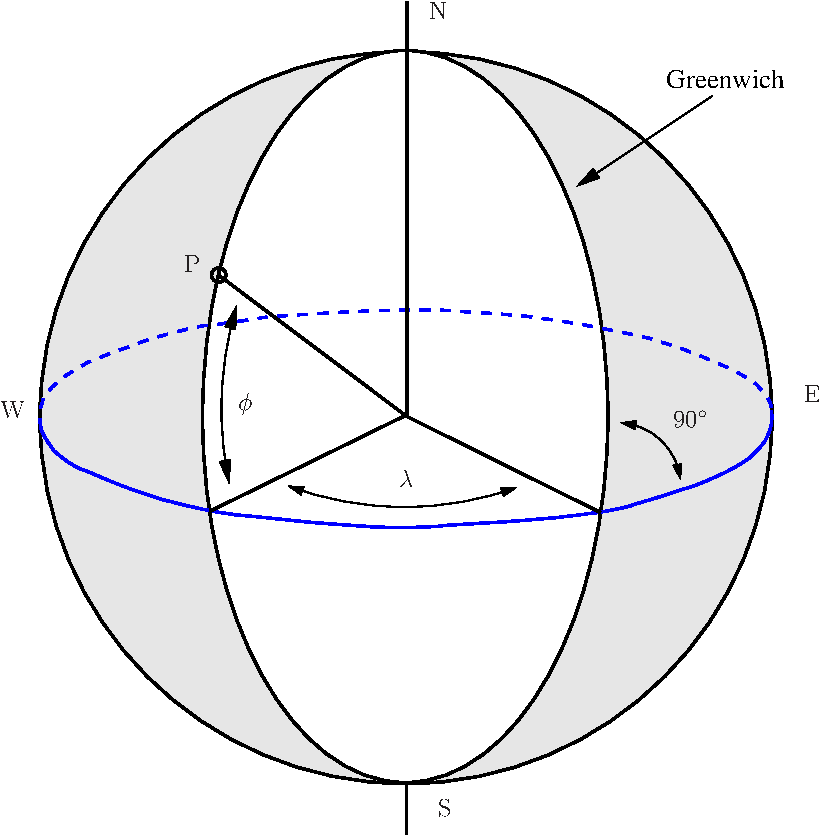
\includegraphics[width=8cm]{../figures/longlat.pdf}
\end{center}
\caption{Illustration av longitud ($\lambda$) och latitud ($\phi$) på
  jorden. Storcirklar som går genom polerna är
  longitudcirklar. Cirklar som är parallella med ekvatorn är
  latitudcirklar. }
\label{figearth}
\end{figure}


\section{Himmelsfären}

\subsection{Ekvatoriella koordinater}

\begin{figure}[ht]
\begin{center}
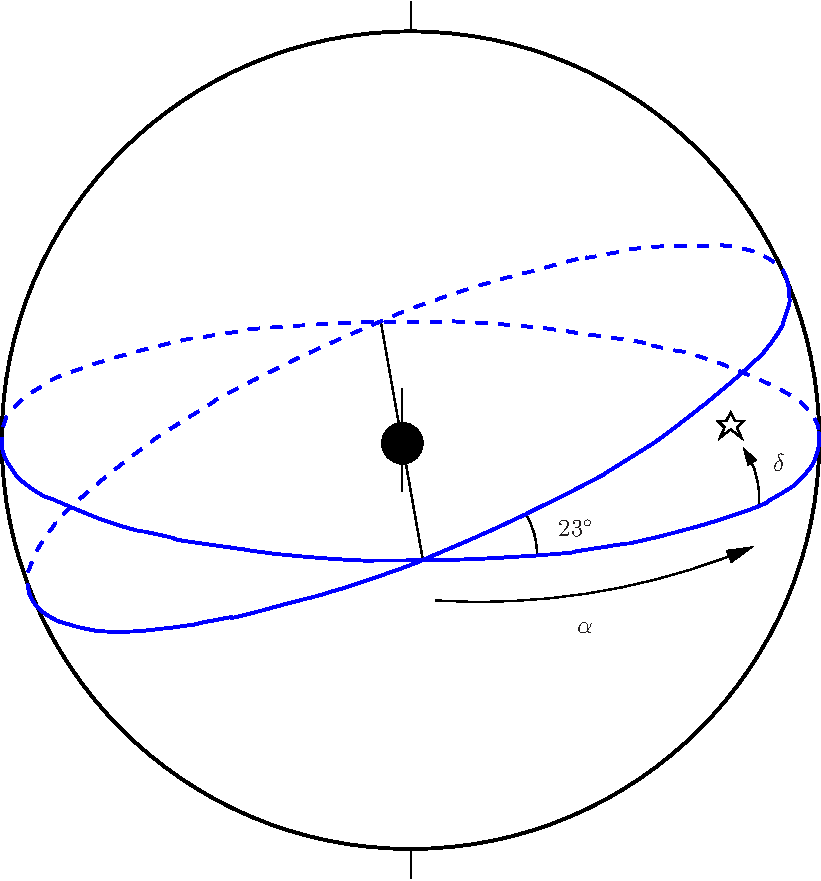
\includegraphics[width=8cm]{../figures/celestial.pdf}
\end{center}
\caption{Det ekvatoriella koordinatsystemet, med RA $\alpha$ och
  deklination $\delta$. Jorden ligger i centrum. Ekliptikans plan
  lutar 23.5$^\circ$ jämfört med jordens ekvator.}
\label{figcelest}
\end{figure}

Himmelsfären är en inbillad sfär som är koncentrisk med Jorden. På
denna sfär är de astronomiska objekten placerade (se
Fig.~\ref{figcelest}). Himmelsekvatorn är de naturliga förlängningen
av jordekvatorn. Eftersom jordens rotationsaxel lutar 23.5 grader
jämfört med solsystemsplanet sammanträffar inte ekliptikan (solens
banplan) med himmelsekvatorn. Punkten där Solen korsar himmelsekvatorn
på väg norrut kallas Vårdagjämningnen och inträffar runt den 21
mars. Då ligger solen i jordens ekvatorialplan och dag och natt är
lika långa. På väg söderut passerar sedan Solen himmelsekvatorn igen
den 21 september (höstdagjämningen). Sommar- och vintersolstånden
inträffar då solen är längst bort från himmelsekvatorn och inträffar
21 juni respektive 21 december.

\medskip
{{$\rightarrow$ Markera norra och södra himmelspolen,
    himmelsekvatorn , ekliptikan, solstånden samt vår- och
    höstdagjämningarna i Fig.~\ref{figcelest}.}}
\medskip

Positioner på himmelssfären definieras av vinklar längs
storcirklar. Himmelslongituden (rektascension, RA) $\alpha$ för ett
astronomiskt objekt definieras i analogi med longitud på jorden. Den
mäts österut från vårdagjämningen längs himmelsekvatorn. RA uttrycks i
timmar, minuter och sekunder där 24 timmar motsvarar hela varvet,
360$^\circ$.

I analogi med latitud definieras himmelslatitud (deklinationen) som
vinkelavståndet till ett objekt från himmelsekvatorn. Tillsammans
bestämmer RA och deklinationen fullständigt en posiition på
himmelssfären.

Tänk dig nu att vi befinner oss på en plats $P$ på jorden vid
latituden $\phi$, och att vi vill observera himlen. Ett astronomiskt
objekt med deklinationen $\delta$ når då sin maximala höjd över
horisonten $h_{\rm max}$, och minimala höjd $h_{\rm min}$ enligt

\begin{equation}
\begin{array}{l}
h_{\rm max} = 90^\circ -|\phi-\delta| \\
h_{\rm min} = -90^\circ +|\phi+\delta|. 
\end{array}
\end{equation}

{{$\rightarrow$ I Onsala stannar alltid astronomiska
    objekt med $\delta > 33^\circ$ 
alltid över horisonten (de är circumpolära); }}

{{$\rightarrow$ de med $\delta < -33^\circ$ kommer aldrig
    över horisonten.}}


\subsection{Den lokala stjärntiden}

\begin{figure}[ht]
\begin{center}
 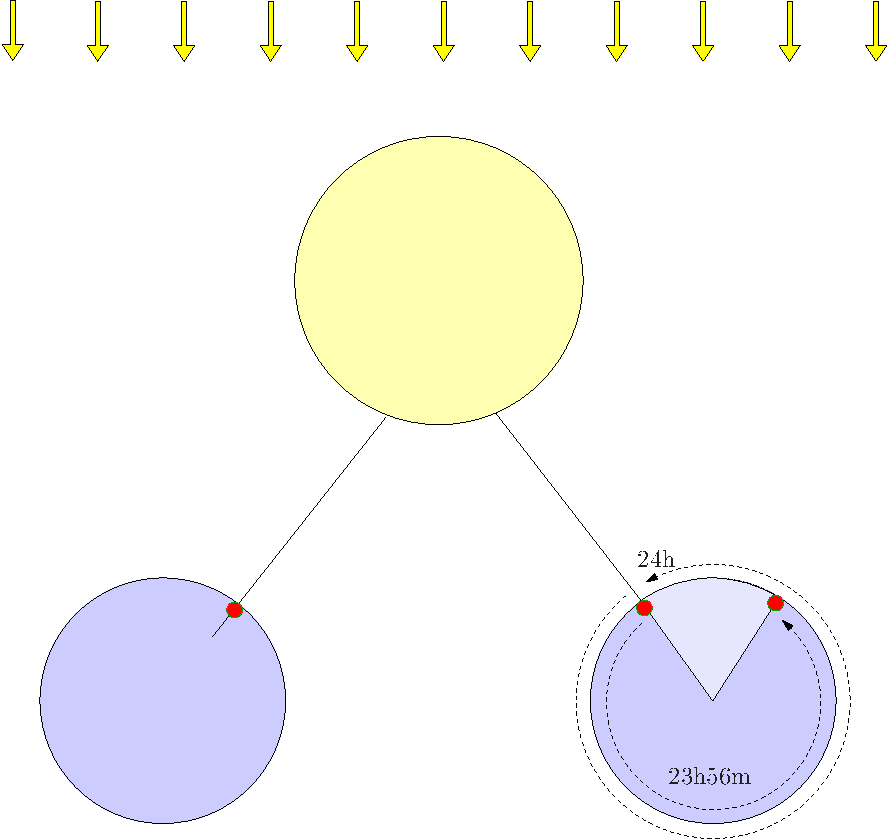
\includegraphics[width=8cm]{../figures/lst.pdf}
\end{center}
\caption{Den lokala stjärntiden (LST) är definierad relativt
  stjärnorna, medan soltiden definieras relativt solen. 24~timmar
  LST-tid motsvarar bara 23~timmar 56~minuter 05~sekunder soltid.}
\label{figlst}
\end{figure}

Anledningen till att man mäter RA österut är att det gör himmelsfären
till en urtavla. Visaren är den \textbf{lokala meridianen} (nord-syd
linjen som går genom observatörens zenith).


Vid vårdagjämningen är den lokala stjärntiden (LST) 0 timmar. Detta
inträffar klockan tolv (soltid).

När tiden går kommer astronomiska objekt på den lokala meridianen ha
en större RA. Vid varje tillfälle och vid varje plats på jorden är
alltid LST lika med RA för de astronomiska objekten på den lokala meridianen.

``Himmelsklockan'' går fortare än solklockan varje dag. Detta kommer
sig av att jorden roterar både runt sin egen axel och runt solen,
vilket illustreras i figur~\ref{figlst}. Efter 24 timmar soltid har en
plats på jorden samma soltid igen (ett dygn). Men 24 timmar stjärntid
går ungefär fyra sol-minuter fortare, eftersom vi inte behöver vrida
oss lika långt för att komma till samma position relativt
stjärnorna. 24 timmar LST motsvarar därför 23 timmar 56 minuter och 5
sekunder soltid. Varje dag inträffar en LST tid fyra minuter (soltid)
tidigare än dagen innan.

Vid vårdagjämningen är alltså LST 0h vid soltiden 12h. Nästa dag vid
12h soltid är LST 0h 3min 56s. För varje månad inträffar en LST tid 2
timmar tidigare.

\subsection{Hur kan jag veta om min källa är synlig?}
\label{app:visiblecoords}

Anta att vi vill observera i en viss riktning i det galaktiska planet
(en viss longitud $l$ och latitud $b=0$), vid en viss tidpunkt.

Först måste vi konvertera Våra galaktiska koordinater till
ekvatoriella koordinater (RA \& DEC). För att förenkla har vi räknat
ut RA \& DEC för ett antal galaktiska longituder i planet. Dessa finns i tabell \ref{tab:radec}. 

Som vi redan sett kan man inte observera källor som alltid ligger under
horisonten i Onsala (de med $\delta < -33^\circ$).

Det bästa sättet att lära sig hur det fungerar är att studerar några exempel!

\bigskip {\bf Example~1.} Idag är julafton och jag har tillgång till
ett litet optiskt teleskop. Jag skulle vilja observera den vackra
``virvelgalaxen'' M51. Är det möjligt? 

\smallskip M51 har koordinaterna $\alpha\simeq13$~h~30m,
$\delta\simeq+47^\circ$. Det betyder att M51 kommer att vara som högst
över horisonten vid LST=13~h~30.

LST= 0~h vid = 12~h den 21 mars.

LST= 0~h vid $12-(2\times 9) = -6$~h (eller $24-6=18$~h) runt 21 dec
eftersom det är nio månader efter den 21 Mars, och LST går 2 timmar
fortare varje månad.

LST=13~h~30 vid 18+13~h~30= 7~h~30.

M51 kommer att vara som högst på himlen på morgonen klockan 7h30 och
kommer att stiga under den andra delen av natten,

\begin{table}
\label{tabcoord}
\begin{center}
\begin{tabular}{rrr}
\hline
\medskip
$l$ & $\alpha(J2000)$ &$\delta(J2000)$\\
$^\circ$ &h m &$^\circ\,\,\,\,\,$$'$\\
\hline
0 & 17h45 & --28:56 \\
20 & 18h27 & --11:29 \\
40 & 19h04 & 06:17 \\
60 & 19h43 & 23:53 \\
{\bf\green 80}  & 20h35 & 40:39\\
{\bf\green 100} & 22h00 & 55:02\\
{\bf\green 120} & 00h25 & 62:43 \\
{\bf\green 140} & 03h07 & 58:17 \\
{\bf\green 160} & 04h46 & 45:14\\
180 & 05h45 & 28:56\\
200 & 06h27 & 11:29\\
220 & 07h04 & --06:17\\
240 & 07h43 & --23:53\\
\red 260 & 08h35 & --40:39\\
\red 280 & 10h00 & --55:02\\
\red 300 & 12h25 & --62:43\\
\red 320 & 15h07 & --58:17\\
\red 340 & 16h46 & --45:14\\
\hline
\end{tabular}
\caption{Konversion mellan galaktiska koordinater till ekvatoriella
  koordinater för olika $l$ med $b=0$. Longituderna i grön fetstil är
  cirkumpolära i Onsala, och de i rött kommer aldrig över horisonten.
\label{tab:radec}
}
\end{center}
\end{table}
